% !TEX root = rob1.tex
\chapter{Bahnsteuerung}

\section{Grundlagen}
\mparagraph{Trajektorie}
Bewegung eines Roboters aufgefasst als Zustandsänderung über die Zeit,
relativ zu einem stationären Koordinatensystem mit Einschränkungen (Zwangsbedinungen,
Gütekriterien, Neben und Randbedinungen)

\mparagraph{Koordinatensysteme}
\begin{table}[h!]
\centering
\begin{tabular}{ll}
\textbf{Kartesischer Raum}                                                                                                                                                                                                                                                                                                                 & \textbf{Gelenkwinkelraum}                                                                                                                                                                                                                                                                                                                                             \\
\begin{tabular}[c]{@{}l@{}}Näher an der zu lösenden Aufgabe\\ \\ Angabe der Trajektorie erfolgt als
    \\ Funktion der Zustände des Roboters\\ \\ + Bahn einfacher zu formulieren\\ + Interpolation ist
     einfacher\\ - Inverse Kinematik für jeden\\ Trajektorienpunkt zu lösen\\ - Geplante Trajektorie
      nicht immer\\ ausführbar\end{tabular} & \begin{tabular}[c]{@{}l@{}}Näher an der Ansteuerung der
       Teilsysteme\\ des Roboters\\ \\ Bahnsteuerung als Funktion der Gelenkwinkelzustände\\ \\ +
       Ansteuerung der Gelenke ist einfacher\\ + Trajektorie ist eindeutig und berücksichtigt die \\
       Gelenkwinkelgrenzen\\ - Interpolation für mehrere Gelenke\\ - Formulieren der Trajektorie
       umständlicher\end{tabular}
\end{tabular}
\end{table}

\section{Interpolation}
\subsection{Punkt-zu-Punkt , PTP}
\mparagraph{PTP Asynchron/Synchron}
\begin{compactitem}
    \item asynchron: Jedes Gelenk wird sofort mit maximalen Beschleunigung angesteuert. Jede Gelenkbewegung endet
    unabhängig von den anderen. \\
    \item synchron:Alle Gelenke beginnen und beenden ihre Bewegungen gemeinsam
\end{compactitem}
\begin{figure}[!h]
    \centering
    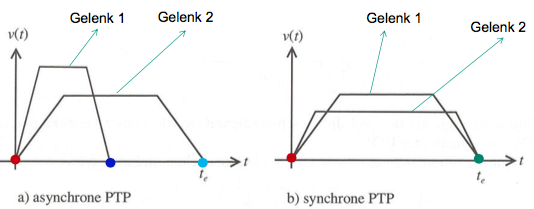
\includegraphics [scale=0.8]{sync}
\end{figure}
\mparagraph{Ablauf}
\begin{compactitem}
    \item Fahrzeit $t_e$
    \item Beschleunigsungszeit $t_b$
    \item Beginn der Bremszeit $t_v$
    \item $s(t_e) = s_e = |q_z - q_{st}|$
\end{compactitem}
\mparagraph{Rampenprofil}
Phase der Beschleunigung
\begin{align}
    t_B &= \frac{v_m}{b_m}\\
    \ddot{s}(t) &= b_m \text{  } 0 \leq t \leq t_b \\
    \dot{s}(t) &= b_mt\\
    s(t) &= \frac{1}{2}b_mt^2
\end{align}
Phase der gleichmäßigen Fahrt
\begin{align}
    \ddot{s}(t) &= 0 \text{  }t_b\leq t \leq t_v\\
    \dot{s}(t) &= v_m\\
    s(t) &= v_mt - \frac{1}{2}b_mt_b^2 = v_mt - \frac{1}{2}\frac{v_m^2}{b_m}
\end{align}
Phase des Bremsvorganges
\begin{align}
    \ddot{s}(t) &= -b_m \text{  } t_v\leq t \leq t_e \\
    \dot{s}(t) &= v_m - b_m(t-t_v)\\
    s(t) &= v_m(t_e - t_b) - \frac{b_m}{2}(t_e-t)^2
\end{align}
Berechnung der Fahrtzeit
\begin{displaymath}
     t_e = \frac{s_e}{v_m} + t_b = \frac{s_e}{v_m} + \frac{v_m}{b_m}
\end{displaymath}
Zeitoptimale Bahn (falls $v_m$ zu groß in Bezug auf Beschleunigung und Bahnlänge)
\begin{displaymath}
     s_e = t_b \cdot v_{m,\text{max}} =  \frac{v_{m,\text{max}}^2}{b_m} \rightarrow
     v_{m,\text{max}} = \sqrt{b_ms_e}
\end{displaymath}

Vorgehen Synchrone PTP:\\
\begin{compactitem}
    \item Bestimme für jedes Gelenk i die PTP Parameter ($s_{e,i}, v_{m,i}, b_{m,i}m, t_{e,i}$)
    \item Bestimmte $t_e = t_{e,\text{max}} = \max{t_{e,i}}$. Achse mit max. Fahrzeit ist Leitachse
    \item Setzte $t_{e,i} = t_e$ für \textbf{alle} Gelenke
\end{compactitem}
\mparagraph{Sinoidbahn}
Phase der Beschleunigung (rest ableiten)
\begin{displaymath}
     s(t) = b_m(\frac{1}{4}t^2 +\frac{t_b^2}{8\pi^2}(\cos(\frac{2\pi}{t_b}t)-1))
\end{displaymath}

Aus $\dot{s}t(b) = b_m\frac{1}{2}t_b = v_m$ folgt $t_b = \frac{2v_m}{b_m}$\\
Phase der gleichmäßigen Fahrt (rest ableiten)
\begin{displaymath}
     s(t) = v_m(t-\frac{1}{2}t_b)
\end{displaymath}
Bremsforgang\\
\textit{fuck this}\\


Berechnung der Fahrtzeit
\begin{displaymath}
     t_e = \frac{s_e}{v_m} + t_b = \frac{s_e}{v_m}+ \frac{2v_m}{b_m}
\end{displaymath}
\subsection{Linear und Zirkularinterpolation}

\subsection{Splineinterpolation}
\section{Approximierte Bahnsteuerung}
\subsection{Bezierkurven}
Verlaufen im Unterschied zu kubischen Splines nicht durch alle Stützpunke. Werden nur beeinflusst.
\subsection{De Casteljau Algorithmus}
Annäherung an Bezierkurven. Effiziente Berechung und Näherungsdarstellung durch einen
Polygonzug.

\begin{compactitem}
    \item Gegeben: n Kontrollpunkte $P_0, ..., P_{n-1}$
    \item Start: $P_i^0 = P_i$
    \item Iteration k: $P_i^{k+1} = (1-t_0)P_i^k + t_oP_{i+1}^k$
\end{compactitem}
